% Corridor Reuse Outperforms Bathymetry in Submarine Cable Route Prediction
%
% BUILD:  pdflatex main -> bibtex main -> pdflatex main -> pdflatex main
%         (or: latexmk -pdf main)
%
% VENUE.  Set for an IEEE journal (IEEE Access, IEEE J. Ocean. Eng., IEEE
% Systems Journal). For a conference, change the class option below to
% [conference] -- IEEEtran handles both -- and cut Sections VI-B, VII-C and
% Tables VI and IX, which are the parts that exist to survive a journal
% reviewer rather than to carry the argument.
%
% NUMBERS.  The tables and the \n... macros are generated from the analysis
% cache by scripts/research/make-paper-tables.mjs. Every headline figure -- the
% abstract, and each claim the argument rests on -- is a macro, so it cannot
% drift from the data. Secondary values quoted in prose are read off the
% generated table on the same page rather than macro'd individually; that keeps
% the source readable, at the cost of a check the generator cannot do for you.
% If you change an analysis, re-run the generator and then re-read the prose.
%
% BEFORE COMPILING:  node scripts/research/make-paper-tables.mjs
%                    node scripts/research/svg-to-pdf.mjs
%                    node scripts/research/check-paper.mjs
\documentclass[journal]{IEEEtran}

\usepackage[T1]{fontenc}
\usepackage[utf8]{inputenc}
\usepackage{graphicx}
\usepackage{booktabs}
\usepackage{amsmath,amssymb}
\usepackage{url}
\usepackage[hidelinks]{hyperref}
\usepackage{cite}

\graphicspath{{figures/}}
% Generated by scripts/research/make-paper-tables.mjs -- do not edit.
% Every inline number in main.tex comes from here, so the prose cannot drift
% from the cache without the build noticing.
\newcommand{\nBathyRoutes}{355}
\newcommand{\nCorpusKm}{206,175}
\newcommand{\nCorpusRoutes}{412}
\newcommand{\nCorridorCtl}{29}
\newcommand{\nCorridorCtlN}{182}
\newcommand{\nCorridorCtlPct}{74}
\newcommand{\nCorridorRaw}{68}
\newcommand{\nDiscGap}{2.63}
\newcommand{\nDiscPairs}{51}
\newcommand{\nDiscretisation}{7.85}
\newcommand{\nErAbove}{33}
\newcommand{\nErBelow}{86}
\newcommand{\nErN}{348}
\newcommand{\nErRho}{0.656}
\newcommand{\nErZ}{12.2}
\newcommand{\nFishSamples}{10,450}
\newcommand{\nFishUsablePct}{82.2}
\newcommand{\nGateDepth}{98}
\newcommand{\nGateRelief}{55}
\newcommand{\nGateRoutes}{235}
\newcommand{\nGateSlope}{47}
\newcommand{\nLocalN}{342}
\newcommand{\nLongHaulP}{\ensuremath{3\!\times\!10^{-4}}}
\newcommand{\nLongHaulWin}{15/15}
\newcommand{\nPlaceboDepth}{+0.42}
\newcommand{\nPlaceboRough}{\ensuremath{-}1.54}
\newcommand{\nPlaceboSlope}{\ensuremath{-}1.65}
\newcommand{\nRegBoth}{6.4}
\newcommand{\nRegCorridor}{6.9}
\newcommand{\nRegFitted}{7.1}
\newcommand{\nRegGeodesic}{7.1}
\newcommand{\nRegHandset}{7.9}
\newcommand{\nRegN}{217}
\newcommand{\nRegSeapath}{9.7}
\newcommand{\nRegSlope}{7.3}
\newcommand{\nTgSystems}{724}


% IEEEtran sets \paragraph as a run-in heading; nothing else is redefined.
\begin{document}

\title{Corridor Reuse Outperforms Bathymetry in\\
Submarine Cable Route Prediction: A Controlled\\
Evaluation on \nCorpusRoutes{} As-Laid Routes}

\author{Pavitra~Sharma% <-- add co-authors here
\thanks{% TODO: affiliation and postal address before submission.
The author is with [Affiliation], [City], [Country]
(e-mail: pavitrasharma2306@gmail.com).}%
\thanks{Analysis code and the full reproduction pipeline are available at
\url{https://github.com/ixpavi/subsea-siting}.}}

\markboth{IEEE Journal (preprint)}%
{Sharma: Corridor Reuse Outperforms Bathymetry in Submarine Cable Route Prediction}

\maketitle

\begin{abstract}
Submarine cable route planning tools---academic, commercial and
patented---optimise a least-cost path over seabed terrain, on the premise that
real cable routes are largely the outcome of such an optimisation. That premise
is widely assumed and, to our knowledge, never measured against cables that
were actually laid. We assemble a corpus of \nCorpusRoutes{} as-laid routes
(\nCorpusKm{}\,km) republished by seven national hydrographic offices, of which
\nBathyRoutes{} have matched bathymetry, and evaluate against grids at 460\,m
and 1.85\,km. Three controls carry the evaluation: a
\emph{placebo-displaced} baseline that establishes what each instrument reads
when no preference exists, a \emph{discretisation} control that measures what a
grid search costs before it is compared with an analytic baseline, and a
\emph{resolution gate} that quantifies the sensitivity lost when the grid is
coarsened. Terrain preference is real but small---slope
\nPlaceboSlope{} percentile points against the placebo---and although adding it
to a least-cost search cuts median prediction error from \nRegSeapath{}\,km to
\nRegFitted{}\,km, \emph{fitting} the cost weights does not beat guessing them.
A competing signal is markedly stronger. Cables sit \nCorridorCtl\% closer to
other operators' cables than displaced controls do, on \nCorridorCtlPct\% of
routes, after excluding same-agency data, the landfall approaches and every
cable sharing a named landing point. Built into the same search, this corridor
term is the only method tested that beats a great circle, and it
\emph{strengthens} with route length, winning on \nLongHaulWin{} routes above
2{,}000\,km ($p=\nLongHaulP$). Its operating range is predictable: a per-route
rule (Spearman $\rho=\nErRho$, $n=\nErN$) states in advance when it will fail.
A third candidate driver, fishing effort, shows no signal once landfalls are
removed. Terrain-driven route optimisation models the weaker of two available
signals while ignoring the stronger one, which requires no bathymetry at all.
\end{abstract}

\begin{IEEEkeywords}
Submarine cables, route planning, least-cost path, model validation, spatial
statistics, placebo control, bathymetry, marine spatial planning.
\end{IEEEkeywords}

\section{Introduction}
\IEEEPARstart{S}{ubmarine} telecommunications cables carry almost all
intercontinental data traffic, and where one is laid determines its cost, its
permitting burden and its exposure to the hazards that will eventually break
it. The dominant computational approach to choosing that path is the
least-cost path: rasterise the seabed, assign each cell a cost from depth,
slope, roughness and a hazard term, and search for the cheapest route between
two landing points~\cite{wang2019cost,wang2018fastmarching,makrakis2023gis,
wang2020trunkbranch}. Commercial packages implement the same
idea~\cite{makaiplan}, and a granted patent extends it by \emph{learning} the
cost surface from bathymetry around existing routes~\cite{google_patent_2021}.

Every one of these rests on a premise: that the position of a real submarine
cable is substantially explained by seabed terrain. The premise is rarely
stated and, as far as we can establish, never measured. The most recent
comparative study of cable path planning algorithms evaluates Fast Marching, a
Dijkstra variant and a great circle against \emph{modelled cost}, describes its
own output as ``an initial guideline or benchmark rather than the final
route'', and reports no accuracy metric against any deployed
cable~\cite{wang2024evaluating}. A GIS multi-criteria study applied to real
case studies likewise reports no comparison with the cables actually
laid~\cite{makrakis2023gis}. The patent trains a model on existing routes
precisely \emph{because} it assumes those routes optimise over bathymetry, and
reports no validation of that assumption~\cite{google_patent_2021}.

This paper supplies the missing measurement, and finds that the premise is
weak.

\subsection{Why the measurement is harder than it looks}
Three properties of this problem defeat a naive evaluation, and each produced a
wrong headline in our own work before it was controlled for.

\emph{The null is not where you think it is.} Seabed terrain is strongly
spatially autocorrelated. Any line drawn on it---cable or not---will score off
the nominal midpoint of a local distribution, so a percentile near 50 cannot be
read as ``no preference'' without measuring what a non-cable reads.

\emph{The baseline is not on the same footing.} A great circle is a smooth
analytic curve; a grid search is not. Comparing them attributes the cost of
discretisation to the cost function.

\emph{The instrument changes when the problem does.} Long-haul routing cannot
be searched at the resolution regional routing can, so the grid must coarsen,
and a null result on a coarser grid is indistinguishable from an instrument too
blunt to see the effect.

\subsection{Contributions}
\begin{enumerate}
\item \textbf{A validation of the least-cost-path premise against as-laid
routes.} On \nCorpusRoutes{} routes from seven national hydrographic offices,
we report prediction error in kilometres against the cable actually laid, for
six methods sharing one search, one grid and one endpoint treatment
(Section~\ref{sec:prediction}).

\item \textbf{Three transferable controls}---placebo displacement, a
discretisation penalty, and a resolution gate---each of which changed a
headline here (Section~\ref{sec:method}). We claim the \emph{transfer and the
measured consequence of omitting them}, not the designs; Section~\ref{sec:rw}
gives their homes in other literatures.

\item \textbf{A stronger, bathymetry-free signal.} Corridor reuse survives
same-agency exclusion, landfall trimming, shared-landing-point exclusion, and
complete replacement of the candidate set, and it strengthens with route length
(Sections~\ref{sec:corridor}--\ref{sec:candidates}).

\item \textbf{A rule that predicts its own failure.} Corridor following helps
only when the neighbour geometry's error is small relative to the prediction's
scale; tested per route it is monotonic across six bins
(Section~\ref{sec:ratio}).

\item \textbf{A tested and rejected alternative explanation.} Fishing effort,
the mechanism behind most cable faults, shows no relationship to cable position
once landfalls are removed (Section~\ref{sec:fishing}).
\end{enumerate}

\section{Related Work}\label{sec:rw}

\subsection{Least-cost-path cable routing}
Least-cost path and A$^\star$ over a rasterised cost surface is textbook, and
its application to submarine cables is a small but active literature dominated
by one group~\cite{wang2018fastmarching,wang2019cost,wang2020trunkbranch,
wang2023tonga,wang2024evaluating}. Multi-criteria decision analysis over
normalised weighted criteria is likewise standard, and has been applied to
cable siting with seismic fault avoidance~\cite{makrakis2023gis}.

\emph{Nothing in this paper claims a new routing algorithm.} Our search is
deliberately conventional; it exists so that the premise under test has a
concrete instance. These are well-built optimisers whose objective function has
not been checked against reality---a gap their authors state
themselves~\cite{wang2024evaluating}---rather than incorrect ones.

\subsection{Learning route cost from observed paths}
US~11,031,757~B2~\cite{google_patent_2021} claims generating cable routes from
a model trained on bathymetry and existing route data. It is prior art for
\emph{learning a cost surface}, which is therefore not claimed here. It is also
the strongest available argument that the question matters: a major operator
built machinery on the assumption that existing routes encode bathymetric
optimisation, without publishing a test of it.

\subsection{What is not claimed as novel}
Comparing an observed path against displaced alternatives that share its
geometry is the foundational design of step-selection analysis in movement
ecology---a matched case--control used-availability
design~\cite{fortin2005wolves,thurfjell2014ssf,avgar2016issa}. The
shift-and-rotate null model~\cite{ridder2024shiftrotate} is closer still: it
preserves a predictor's spatial structure while destroying its alignment with
the response, which is exactly the logic of displacing a cable sideways. We
claim the transfer to \emph{engineered linear infrastructure} and the measured
consequence of omitting it, not the design. A known caveat transfers with it:
such nulls are sensitive to linear trend~\cite{wagner2015moran}, and a control
displaced along a heading may inherit a depth gradient---which is why
Section~\ref{sec:localpref} reports depth separately and finds it moves the
other way.

Likewise, reporting the share of admissible weightings under which a
recommendation holds is rank acceptability analysis, which has a name and a
literature~\cite{lahdelma1998smaa,lahdelma2001smaa2}.

\section{Data}\label{sec:data}

\subsection{As-laid routes}
The geometry published on cable maps is schematic. Measured directly, a
widely used commercial dataset~\cite{telegeography} carries 7.3 vertices per
1{,}000\,km, a median segment of 69\,km, and a longest single segment of
5{,}650\,km. A 5{,}650\,km straight line records that two places are connected,
not where the cable goes; it cannot support any claim about route position.

We therefore use EMODnet Human Activities~\cite{emodnet_humanactivities}, which
republishes cable positions from national hydrographic offices---the data
fishermen and marine planners use to avoid them. Telecommunication layers only;
power cables have different burial rules and route economics. Screening for
routes long enough to have had alternatives and sampled finely enough to show
which was taken ($\geq 25$\,km, $\geq 50$ vtx/1{,}000\,km) gives
\nCorpusRoutes{} routes and \nCorpusKm{}\,km (Table~\ref{tab:corpus}).

The corpus is Europe-weighted but not shelf-limited: the French SHOM layer
covers overseas territories, reaching the Pacific, Indian Ocean and Caribbean.
Median depth along the corpus is 64\,m, but 17\% lies below 2{,}000\,m and 4\%
is abyssal, to a maximum of 5{,}272\,m. Deep-water routing decisions are
present.

\begin{table}[t]
\caption{As-laid route corpus by publishing agency. Sampling fidelity spans a
factor of 30, which \S\ref{sec:dose} shows is confounded with terrain.}
\label{tab:corpus}
\centering\footnotesize
\begin{tabular}{@{}lrrrr@{}}
\toprule
Source & Routes & km & vtx/1{,}000\,km & Median seg. \\
\midrule
DE BSH-CONTIS & 23 & 2,224 & 3,369 & 6\,m \\
UK OGA & 2 & 130 & 692 & 327\,m \\
NL Rijkswaterstaat & 94 & 20,398 & 378 & 703\,m \\
FR SIGCables & 52 & 23,147 & 168 & 2.49\,km \\
FR SHOM & 217 & 156,153 & 148 & 2.11\,km \\
MT IOI-MOC & 5 & 845 & 91 & 3.07\,km \\
ES CICA & 19 & 3,278 & 89 & 6.02\,km \\
\midrule
\textit{TeleGeography} & \textit{724} & \textemdash & \textit{7.3} & \textit{69\,km} \\
\bottomrule
\end{tabular}
\end{table}


\subsection{Bathymetry}
Two grids are used, and they are not interchangeable.

\emph{460\,m}, downsampled from EMODnet Bathymetry DTM at native 1/16
arc-minute ($\sim$115\,m)~\cite{emodnet_bathymetry}, comfortably finer than the
corpus's 2\,km median route sampling---the condition for resolving what routes
bent around. The downsampling was validated rather than assumed: only 0.1\% of
output cells exactly equal a source cell, so the service interpolates rather
than point-samples; global mean signed error is $-1.2$\,m; the residual is
interpolation noise concentrated on steep cells (steep-decile RMS 47\,m)
against relief of thousands of metres. Of \nCorpusRoutes{} routes, 356 fall
inside the product's envelope and one crosses a genuine coverage hole and is
excluded rather than interpolated over, leaving \nBathyRoutes{} routes, which
carry every terrain result below.

\emph{1.85\,km}, a uniform 60~cells/degree grid covering the search corridor of
every corpus route, back-filled from the NOAA NCEI global DEM
mosaic~\cite{noaa_ncei_dem} where EMODnet does not reach.
Section~\ref{sec:longhaul} explains why this grid is unavoidable and
Section~\ref{sec:gate} measures what it costs.

\emph{A data defect worth reporting.} EMODnet encodes out-of-coverage as
exactly $0$ rather than as a nodata sentinel: 4.85\% of cells across the tiles
we built, with 36 tiles entirely zero, among them Barbados and a mid-Atlantic
block that are simply outside the DTM. NOAA's exact-zero rate on the same
footprint is 0.03\%, i.e.\ genuine sea level. Averaged into a block mean this
fabricates a shallow shelf where there is no data; and because depth is read as
null for any elevation $\geq 0$, such a cell reads as \emph{land}, so a router
treats open Atlantic as coastline and confidently goes around it. We discarded
2{,}203{,}460 such cells and back-filled them. Once the fill is excluded the two
products agree where both report seabed---mean signed difference $+5.0$\,m,
median $|$difference$|$ 18\,m---against an apparent $-1{,}550$\,m disagreement
before it was excluded.

\subsection{Fishing effort}
EMODnet Human Activities vessel density, fishing subset, AIS-derived at
$\sim$1.7\,km native resolution, hours per km$^2$ per month, 2022
epoch~\cite{emodnet_vesseldensity}. Global Fishing
Watch~\cite{kroodsma2018gfw} is the citable global source, but its public grid
is $0.1^\circ$ ($\sim$11\,km), which cannot resolve a decision on a 1.85\,km
routing grid. \nFishUsablePct\% of the \nFishSamples{} route sample points are
scoreable; the remainder lie outside coverage, chiefly Pacific and
southern-hemisphere routes.

\section{Method}\label{sec:method}

\subsection{The placebo-displaced control}\label{sec:placebo}
At each point along a route we take a transect perpendicular to the local
heading and ask where the cable sits within it. The measurement is purely
local: no endpoints, no geodesic, no assumption about what the route was for.
Under the null the expected percentile is 50. Each route contributes one number
(the mean of its samples), because adjacent samples share terrain and pooling
them would inflate significance enormously.

The nominal null of 50 is not trustworthy, for the reason given in
Section~I-A. So the identical measurement is repeated on the same routes
displaced sideways by 20 and 50\,km. Displacement is perpendicular to the
\emph{local} heading rather than a rigid translation, so the separation stays
constant along a turning route (Fig.~\ref{fig:placebo}). Displaced lines are
not cables and cannot express engineering preference, but they share shape,
length, heading and terrain---so whatever they score is what the instrument
reads when no preference exists.

\begin{figure}[t]
\centering
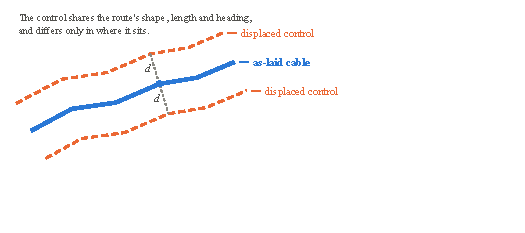
\includegraphics[width=\columnwidth]{fig5-placebo-control.pdf}
\caption{The placebo-displaced control. The control shares the route's shape,
length and heading and differs only in position. Displacement is perpendicular
to the \emph{local} heading, so the separation $d$ is constant along a turning
route.}
\label{fig:placebo}
\end{figure}

\subsection{Route prediction and its baselines}\label{sec:protocol}
Each method is given \emph{only} the two endpoints, predicts the route, and is
scored by the mean distance from the cable actually laid. Every terrain-aware
method uses the same A$^\star$ over the same bathymetry, differing only in cost
weights, so a difference between them cannot come from the search, the grid,
the corridor bound or endpoint handling. Weight fitting uses
leave-one-source-out cross-validation, because routes from one agency share a
sea and a survey convention; a fold is only run where at least eight routes
remain.

\subsection{The discretisation control}\label{sec:disc}
The geodesic is analytic. Every other method is a path over an 8-connected grid
that can step only in $45^\circ$ increments and must snap its endpoints to
water cells. Those are properties of the \emph{search}, not of terrain.

We therefore measure the zero-weight router---terrain entirely ignored, so over
open water it is trying to reproduce the great circle---against the true great
circle, on the \nDiscPairs{} route pairs whose geodesic never touches land. The
median penalty is \nDiscretisation\,km. That handicap is larger than the
\nDiscGap\,km gap between the geodesic and the shortest sea path, so ``A$^\star$
is worse than a straight line'' measures the grid rather than the bathymetry
and cannot support a claim in either direction. Only comparisons between two
grid searches, which share the handicap exactly, are sound.

\subsection{The resolution gate}\label{sec:gate}
A$^\star$ searches a corridor around the endpoints' bounding box, whose area
grows with the \emph{square} of route length. At 240~cells/degree the median
corridor is 478{,}000 cells for a 40--500\,km route and 37.5 million for a
3{,}000\,km one, against a 2{,}000{,}000 expansion cap: long-haul at 460\,m is
not slow, it is impossible.

Coarsening is legitimate only if the instrument can still see the effect. So
the placebo measurement of Section~\ref{sec:placebo} was re-run at
\emph{both} resolutions on the same \nGateRoutes{} routes before any long-haul
number was quoted (Table~\ref{tab:gate}, Fig.~\ref{fig:gate}). The sign is
preserved throughout and \nGateSlope\%, \nGateRelief\% and \nGateDepth\% of the
slope, relief and depth effects survive. Without this, a long-haul null would
be indistinguishable from an instrument too blunt to see the effect.

\begin{table}[t]
\caption{The resolution gate. The identical placebo measurement at both grid
resolutions on the same 235 routes, reported before any long-haul
result is quoted. Same sign throughout; roughly half the sensitivity survives on
slope and relief, almost all of it on depth.}
\label{tab:gate}
\centering\footnotesize
\begin{tabular}{@{}lrrr@{}}
\toprule
Effect vs.\ placebo & 460\,m & 1.85\,km & Retained \\
\midrule
Slope & $-$17.47 & $-$8.24 & \textbf{47\%} \\
Relief & $-$21.33 & $-$11.80 & \textbf{55\%} \\
Depth & $-$7.55 & $-$7.39 & \textbf{98\%} \\
\bottomrule
\end{tabular}
\end{table}


\begin{figure}[t]
\centering
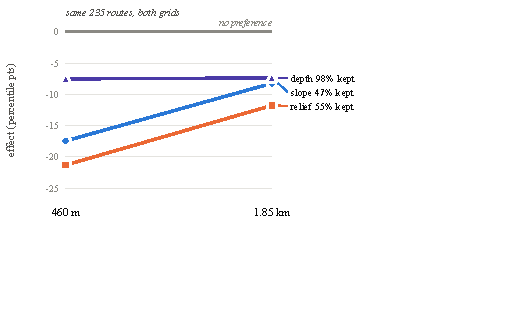
\includegraphics[width=\columnwidth]{fig4-resolution-gate.pdf}
\caption{The resolution gate: the same placebo measurement at both resolutions
on the same routes. Depth survives almost intact; slope and relief lose about
half. Had these collapsed toward zero, every long-haul result would be
uninterpretable rather than negative.}
\label{fig:gate}
\end{figure}

\subsection{Statistics}
All significance is by permutation or sign test on per-route values; no
distributional assumption is made about these heavily skewed quantities.
Percentiles for the zero-inflated fishing surface use midranks, so a cable with
both its controls in empty water scores 50 rather than 0.

\section{Results}

\subsection{Cables do not go straight}
If cables essentially went straight there would be nothing to explain. Median
sinuosity is 1.098 and median maximum lateral departure 17.5\,km. However, 218
of 353 routes have geodesics that cross land: those cables \emph{had} to bend,
and ``cables avoid continents'' is true, trivial, and not a finding.
Restricting to the 135 routes whose straight line was navigable open water,
median sinuosity is 1.043 and median maximum departure 9.8\,km.

On that informative subset, four of five terrain measures show nothing. The one
signal is in the steep tail: 90th-percentile slope is lower on the observed
route for 65\% of routes ($p=0.0005$). Depth runs the \emph{opposite} way, with
61\% of observed routes deeper than their straight line---consistent with
following flat-bottomed troughs rather than minimising depth.

\subsection{Local terrain preference is real and small}\label{sec:localpref}
Table~\ref{tab:preference} gives the placebo-corrected result on
$n=\nLocalN$ routes. Cables sit on measurably flatter and less rugged seabed
than control lines drawn beside them---slope \nPlaceboSlope{} and roughness
\nPlaceboRough{} percentile points---and slightly \emph{deeper}.

\begin{table}[t]
\caption{Local terrain preference against the placebo-displaced baseline
(5\,km transects, $n=342$ routes). A percentile below the placebo means
the cable sits on flatter, less rugged, or shallower ground than the water
beside it. The placebo, not 50, is the zero point.}
\label{tab:preference}
\centering\footnotesize
\begin{tabular}{@{}lrrrr@{}}
\toprule
Metric & Real & Placebo & Effect & $p$ \\
\midrule
Slope & 48.56 & 50.20 & \textbf{\ensuremath{-}1.65} & \ensuremath{<10^{-4}} \\
Roughness & 48.77 & 50.30 & \textbf{\ensuremath{-}1.54} & \ensuremath{<10^{-4}} \\
Depth & 50.71 & 50.29 & \textbf{+0.42} & \ensuremath{<10^{-4}} \\
\bottomrule
\end{tabular}
\end{table}


The control changed the conclusion. Raw, the depth effect read $+0.71$ against
a null of 50 and looked substantial; baselined it is \nPlaceboDepth---most of
it was the instrument, not the cables. Across all twelve placebo combinations
the median percentiles sit at 50.0--50.6, eleven of twelve are
non-significant, and the placebo \emph{never} drops below 50 on slope or
roughness. Effects also strengthen monotonically with transect width (raw slope
49.45 / 48.56 / 48.13 at 2 / 5 / 10\,km), which is the gradient a real
mechanism should show, since a wider transect offers more genuinely different
ground to have chosen instead.

\subsection{The dose--response that failed}\label{sec:dose}
If the mechanism is real it should appear where route choice is possible: over
featureless shelf every position for tens of kilometres is equally flat, while
over rugged ground there are real alternatives. Binning by terrain ruggedness
gives a $3.5\times$ ratio between the flattest and ruggedest quartiles, in the
predicted direction.

\emph{It does not hold.} The series is not monotonic, and quoting a ratio from
the two extreme bins of a noisy four-bin series is a number chosen after seeing
it. Testing the trend across all 343 routes gives Spearman $\rho=-0.174$
($p=0.002$)---real but weak. More seriously, it is confounded with data source:
the corpus is seven agencies whose survey fidelity differs by $30\times$
(Table~\ref{tab:corpus}) and which survey different seas. Within each source,
holding fidelity and cartographic convention constant, \emph{no agency reaches
significance} ($\rho$ from $-0.080$ to $-0.226$, all $p>0.05$). All four are
negative, so the direction is consistent, but the gradient is largely
between-source rather than terrain. The hypothesis is not supported.

\subsection{Route prediction, regional}\label{sec:prediction}
Table~\ref{tab:prediction} reports the headline numbers and
Table~\ref{tab:paired} the paired tests that are actually sound.

\begin{table}[t]
\caption{Regional route prediction, 40--500\,km at 460\,m, on
$n=217$ held-out routes. Error is the mean distance from the cable
actually laid, given only the two endpoints. Bold beats the great circle.
Every terrain-aware row carries the 7.85\,km discretisation
handicap of Table~\ref{tab:paired}'s footnote; the great circle does not.}
\label{tab:prediction}
\centering\footnotesize
\begin{tabular}{@{}lrrrr@{}}
\toprule
Method & Median & Mean & p90 & vs.\ GC \\
 & (km) & (km) & (km) & \\
\midrule
Corridor $+$ terrain & \textbf{6.4} & 9.8 & 21.0 & \textbf{\ensuremath{-}9.9\%} \\
Corridor only & \textbf{6.9} & 10.8 & 25.1 & \textbf{\ensuremath{-}3.1\%} \\
Great circle \textit{(no bathymetry)} & 7.1 & 11.2 & 26.3 & +0.0\% \\
Terrain: all terms, fitted & 7.1 & 11.0 & 24.6 & +0.2\% \\
Terrain: slope only & 7.3 & 10.7 & 22.6 & +3.7\% \\
Terrain: all terms, hand-set & 7.9 & 11.2 & 24.9 & +11.7\% \\
Shortest sea path \textit{(terrain ignored)} & 9.7 & 13.6 & 30.3 & +37.2\% \\
\bottomrule
\end{tabular}
\end{table}

\begin{table}[t]
\caption{Paired per-route comparisons, regional band. Sign test on the share of
routes where the first method lands closer to the as-laid cable. These
comparisons are the sound ones: both members share the grid, the search and the
endpoints, so the discretisation handicap cancels.}
\label{tab:paired}
\centering\footnotesize
\begin{tabular}{@{}lrrr@{}}
\toprule
Comparison & $n$ & Better on & $p$ \\
\midrule
Fitted terrain vs.\ shortest sea path & 217 & \textbf{62\%} & \textbf{\ensuremath{7\!\times\!10^{-4}}} \\
Corridor vs.\ shortest sea path & 196 & \textbf{66\%} & \textbf{\ensuremath{<10^{-4}}} \\
Corridor vs.\ \textit{fitted} terrain & 217 & 55\% & 0.135 \\
Corridor vs.\ hand-set terrain & 217 & \textbf{60\%} & \textbf{0.0028} \\
Adding terrain on top of corridor & 217 & 53\% & 0.415 \\
\bottomrule
\multicolumn{4}{@{}p{0.94\columnwidth}@{}}{\vspace{2pt}\footnotesize
Discretisation control: a zero-weight grid search reproducing a known great
circle still lands a median 7.85\,km from it
($n=51$ open-water pairs), which exceeds the
2.63\,km gap the raw table attributes to bathymetry.} \\
\end{tabular}
\end{table}


Read naively, Table~\ref{tab:prediction} says every bathymetry-aware method is
worse than a straight line. \emph{That reading is wrong}, and the
discretisation control of Section~\ref{sec:disc} is why: the
\nDiscretisation\,km grid handicap exceeds the whole geodesic--sea-path gap.
The comparison that survives is between two grid searches, where the handicap
cancels:

\begin{itemize}
\item \textbf{Terrain preference genuinely improves route prediction.} Median
error falls from \nRegSeapath\,km to \nRegFitted\,km---a 26\% reduction---on
62\% of the \nRegN{} held-out routes ($p=0.0007$), across sources the weights
were never fitted on. Slope alone reaches \nRegSlope\,km; the hand-set
combination of all three terms is worse at \nRegHandset\,km.
\item \textbf{Fitting the weights does not beat guessing them}
(55\%, $p=0.14$ against fitted terrain; the fitted-versus-hand-set contrast is
52\%, $p=0.63$). Whatever the terrain signal is, it is coarse enough that a
sensible hand-set weighting captures it---a direct and unflattering finding
about learned cost surfaces for this problem, and one that bears on
\cite{google_patent_2021}.
\end{itemize}

Fitted weights select slope in four of five folds, roughness in one and depth
in three. Slope is the term that transfers, and it is the same term the placebo
test found the strongest effect on, reached by a completely different method.

\subsection{If not terrain, then what?}\label{sec:corridor}
The most plausible alternative is not exotic: cable projects reuse corridors.
Existing routes carry survey data, established permits, known burial conditions
and proven landing approaches, all expensive to obtain afresh.

Using the identical placebo instrument, we measure the median distance from
each route to the nearest \emph{other} cable, then displace and measure again
(Table~\ref{tab:corridor}). Three exclusion strengths guard the obvious
confounds: a neighbouring segment of the same physical cable would make the
result true by construction, and a single agency densely surveying one busy
corridor says nothing about operators reusing \emph{each other's} routes. The
effect survives all three: even when a route may only be compared against
cables published by a different country's hydrographic office, it sits
\nCorridorRaw\% closer than the same line displaced sideways in the same water.

\begin{table}[t]
\caption{Distance to the nearest OTHER cable, real route vs.\ its
placebo-displaced copy, under progressively stricter controls. The first three
rows exclude candidates by identity; the rest remove the landfall geometry that
identity exclusion cannot touch. The bold row is the figure this paper claims.}
\label{tab:corridor}
\centering\footnotesize\setlength{\tabcolsep}{3pt}
\begin{tabular}{@{}lrrrrr@{}}
\toprule
Control & $n$ & Real & Placebo & Closer & $p$ \\
 & & (km) & (km) & on & \\
\midrule
Any other route & 336 & 2.1 & 9.8 & 90\% & \ensuremath{<10^{-4}} \\
Excl.\ same named cable & 336 & 2.2 & 9.9 & 90\% & \ensuremath{<10^{-4}} \\
Excl.\ same agency & 301 & 7.1 & 22.2 & 83\% & \ensuremath{<10^{-4}} \\
\midrule
\quad $+$ trim 10\,km & 227 & 9.3 & 22.7 & 79\% & \ensuremath{<10^{-4}} \\
\quad $+$ trim 30\,km & 183 & 11.6 & 23.6 & 78\% & \ensuremath{<10^{-4}} \\
\quad $+$ trim 50\,km & 158 & 11.5 & 22.3 & 79\% & \ensuremath{<10^{-4}} \\
\midrule
\textbf{\quad $+$ trim 30, excl.\ shared landing} & \textbf{182} & \textbf{19.0} & \textbf{26.6} & \textbf{74\%} & \textbf{\ensuremath{<10^{-4}}} \\
\bottomrule
\end{tabular}
\end{table}


\emph{But identity exclusion is not enough}, and this is where the uncontrolled
figure fails. Cables converge at landing points because they have to. Two
systems making landfall on the same beach are close there for reasons unrelated
to corridor reuse, and a different operator's cable landing beside mine passes
all three exclusions. Because displacement is applied per-vertex, it moves the
real route's endpoints out of those convergence zones, so the real line samples
crowded landfall water while its placebo samples emptier water beside it.

Two further controls are therefore applied, with the placebo receiving
identical treatment. \emph{Trimming the approaches} decays the effect and then
\emph{plateaus} near 50\% (Table~\ref{tab:corridor}); pure landfall geometry
would keep falling toward zero once the trim exceeded a convergence zone's
width. \emph{Excluding cables that land where I land}, using published landing
points as an independent source, is stable across the association radius
(31\%/29\%/26\% at 5/10/20\,km), which is what a real effect looks like and a
threshold artefact does not.

\textbf{So the honest figure is \nCorridorCtl\%, not \nCorridorRaw\%.} Roughly
half the uncontrolled effect was the landfall approaches and a further part was
cables genuinely sharing a landfall. What remains is corridor reuse in open
water, on \nCorridorCtlPct\% of the \nCorridorCtlN{} routes that survive both
controls, at $p<10^{-4}$---still several times the terrain effect, and
requiring no survey data at all.

\subsection{Corridor reuse as a competing router}
Turning the observation into a model, we add a fourth cost term: distance to
the nearest existing cable, zero at a cable and saturating 25\,km away.
Everything else is unchanged. The corridor term is fed a same-agency exclusion,
because a router that can see the route it is predicting traces it and scores
perfectly while measuring nothing.

Corridor following is the first and only method to beat the great circle
(Table~\ref{tab:prediction}: \nRegCorridor\,km alone, \nRegBoth\,km with
terrain, against \nRegGeodesic\,km), and it does so while carrying the same
\nDiscretisation\,km handicap that made that comparison unfair for terrain. It
beats the terrain-free baseline decisively (66\%, $p<10^{-4}$) and hand-set
terrain (60\%, $p=0.003$).

Two cautions belong with that. It is \emph{not} statistically distinguishable
from \emph{fitted} terrain at this sample size (55\%, $p=0.14$). And although
corridor $+$ terrain has the best median, adding terrain wins on only 53\% of
routes ($p=0.42$): terrain helps markedly on some and hurts on others, so the
median moves while the win rate sits at chance. Reporting ``corridor $+$
terrain is best'' on the median alone would overstate what the paired test
supports.

\subsection{Does any of this hold for long-haul cables?}\label{sec:longhaul}
The strongest objection to the above is that it caps routes at 500\,km and sits
inside a regional bathymetry envelope, while the literature it argues with is
about trans-oceanic systems. Testing on one regime and generalising to the
other is a reason to reject, not a limitation to note in passing.

Table~\ref{tab:bands} extends the experiment to every band up to 6{,}400\,km on
the 1.85\,km grid, whose sensitivity cost is quantified in
Section~\ref{sec:gate}; Fig.~\ref{fig:bands} plots the same result relative to
a great circle, and Table~\ref{tab:bandpaired} gives the paired tests.

\begin{table}[t]
\caption{Median prediction error by route length, all bands on the same
1.85\,km grid. Bold is the best method in that band. Corridor following
improves monotonically with length; every terrain variant does not.}
\label{tab:bands}
\centering\footnotesize
\begin{tabular}{@{}lrrrrrr@{}}
\toprule
Band & $n$ & GC & Sea path & Terrain & Corridor & Cor$+$ter \\
 & & \multicolumn{5}{c@{}}{median error (km)} \\
\midrule
40--500\,km & 253 & 7.1 & 9.8 & 8.1 & 6.5 & \textbf{5.8} \\
500--1,000\,km & 47 & 43.1 & 51.6 & \textbf{27.8} & 37.6 & 29.8 \\
1,000--2,000\,km & 28 & 149.4 & 86.1 & 84.3 & 52.7 & \textbf{36.9} \\
2,000+\,km & 15 & 268.3 & 248.0 & 178.6 & \textbf{55.6} & 97.4 \\
\bottomrule
\end{tabular}
\end{table}

\begin{table}[t]
\caption{Paired per-route comparisons within each length band. The natural
objection to a regional corpus predicts corridor following weakening with
distance; it strengthens, and above 2{,}000\,km adding terrain on top of it
reverses sign.}
\label{tab:bandpaired}
\centering\footnotesize\setlength{\tabcolsep}{3pt}
\begin{tabular}{@{}llrrr@{}}
\toprule
Band & Comparison & $n$ & Better on & $p$ \\
\midrule
40--500\,km & Corridor vs.\ terrain & 253 & \textbf{62\%} & \textbf{\ensuremath{3\!\times\!10^{-4}}} \\
 & Corridor vs.\ sea path & 206 & \textbf{71\%} & \textbf{\ensuremath{<10^{-4}}} \\
 & Terrain added to corridor & 232 & 51\% & 0.844 \\
\midrule
500--1,000\,km & Corridor vs.\ terrain & 47 & 49\% & 1.000 \\
 & Corridor vs.\ sea path & 43 & \textbf{74\%} & \textbf{0.0023} \\
 & Terrain added to corridor & 47 & 62\% & 0.145 \\
\midrule
1,000--2,000\,km & Corridor vs.\ terrain & 28 & 68\% & 0.089 \\
 & Corridor vs.\ sea path & 22 & \textbf{86\%} & \textbf{0.0014} \\
 & Terrain added to corridor & 28 & 46\% & 0.850 \\
\midrule
2,000+\,km & Corridor vs.\ terrain & 15 & \textbf{100\%} & \textbf{\ensuremath{3\!\times\!10^{-4}}} \\
 & Corridor vs.\ sea path & 14 & \textbf{93\%} & \textbf{0.0033} \\
 & Terrain added to corridor & 15 & 27\% & 0.121 \\
\bottomrule
\end{tabular}
\end{table}


\begin{figure}[t]
\centering
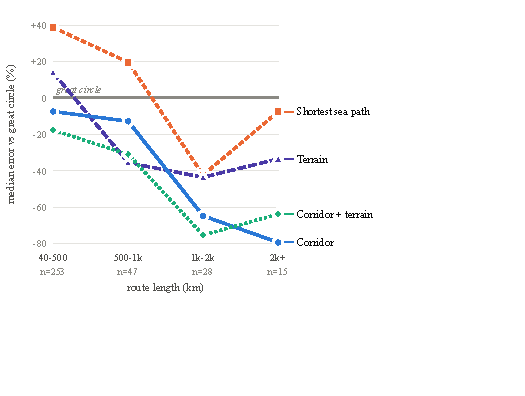
\includegraphics[width=\columnwidth]{fig1-prediction-by-band.pdf}
\caption{Median prediction error relative to a great circle; below the line
beats a straight line. Corridor following improves steadily with route length
while every terrain variant flattens out---the opposite of what an objection to
a regional-only corpus would predict.}
\label{fig:bands}
\end{figure}

A reviewer's natural assumption is that corridor reuse is a shallow-water,
landing-point artefact that will not survive in deep ocean. \textbf{The data
says the reverse.} Corridor following is weakest on the shelf and dominant
trans-oceanically, beating hand-set terrain on \nLongHaulWin{} routes above
2{,}000\,km ($p=\nLongHaulP$) and the shortest sea path on 86\% of
1{,}000--2{,}000\,km routes. Above 2{,}000\,km, adding terrain on top of
corridor actively \emph{hurts} (27\%, $p=0.12$). The regime the method is
marketed for is the regime where it does worst against a bathymetry-free
alternative.

The regional result also replicates at the coarser resolution---corridor
\nRegCorridor{}$\rightarrow$6.5\,km, corridor $+$ terrain
\nRegBoth{}$\rightarrow$5.8\,km, ordering unchanged---so the two grids can be
set side by side rather than silently mixed.

\subsection{Is the corridor result an artefact of a thin candidate set?}
\label{sec:candidates}
It could have been. Corridor distance above is measured against the
\nCorpusRoutes-route corpus under same-agency exclusion, which for a
transatlantic route leaves a handful of European candidates. Measured: the
median distance to the nearest corpus candidate is 7.9\,km at 40--500\,km but
98.1\,km above 2{,}000\,km---beyond the 25\,km saturation scale, so the cost
term is flat across most of the route. The study's strongest result rested on
its sparsest candidate set.

We therefore replace the candidate set entirely with \nTgSystems{}
TeleGeography systems~\cite{telegeography}, which are dense in every band
(5.1--9.2\,km). Two problems had to be solved. Its geometry is schematic, so
paths are densified to 2\,km before indexing---a more \emph{representative}
instrument and a \emph{noisier} one. And the subject cable is in the candidate
set with no agency structure to exclude on. A fixed exclusion radius does not
work here, and finding that out was useful: \emph{no} corpus route has a
TeleGeography system within 5\,km, so a radius tight enough to mean ``this is
the same cable'' fires on nothing, while one loose enough to fire discards
genuine corridor-mates. Systems are therefore ranked by how closely they shadow
the subject and the top $k$ dropped.

\begin{table*}[t]
\caption{Replacing the candidate set. Each cell is median error (km) / share of
routes beating a great circle, for the EMODnet corpus under same-agency
exclusion and for 724 TeleGeography systems with the $k$
closest-tracking systems removed. Bold is significantly better than a great
circle, \underline{underlined} significantly worse. Long-haul survives an
independent candidate set and an unrelated exclusion mechanism; the regional
band does not.}
\label{tab:candidates}
\centering\footnotesize
\begin{tabular}{@{}lrcccc@{}}
\toprule
Band & $n$ & Corpus & TG $k{=}0$ & TG $k{=}1$ & TG $k{=}3$ \\
\midrule
40--500\,km & 259 & 6.4 \,/\, \textbf{57\%} & 7.3 \,/\, 52\% & 11.0 \,/\, \underline{36\%} & 12.3 \,/\, \underline{32\%} \\
500--1,000\,km & 47 & 37.6 \,/\, 57\% & 28.5 \,/\, 64\% & 39.0 \,/\, 53\% & 39.1 \,/\, 55\% \\
1,000--2,000\,km & 28 & 52.7 \,/\, \textbf{82\%} & 36.2 \,/\, \textbf{79\%} & 63.0 \,/\, \textbf{79\%} & 79.7 \,/\, \textbf{75\%} \\
2,000+\,km & 15 & 55.6 \,/\, \textbf{100\%} & 130.1 \,/\, \textbf{100\%} & 149.6 \,/\, \textbf{100\%} & 155.5 \,/\, \textbf{100\%} \\
\bottomrule
\end{tabular}
\end{table*}


Table~\ref{tab:candidates} gives the result. \textbf{Long-haul survives}: an
independent candidate set, an unrelated exclusion mechanism and the three
closest-tracking systems removed, and corridor following still beats a great
circle on 75\% of 1{,}000--2{,}000\,km routes and 15/15 above 2{,}000\,km.
\textbf{Regionally it fails.} The reason is measurable rather than mysterious,
and it is the subject of the next section.

\subsection{The error-ratio rule}\label{sec:ratio}
Across bands, the ratio of the neighbour geometry's error to the great circle's
error is 1.76 regionally (where corridor following hurts) and 0.17--0.18
long-haul (where it helps). A corridor known only to $\pm12$\,km cannot improve
a 7\,km prediction. This also explains why the surveyed corpus beats
TeleGeography at 2{,}000$+$\,km despite near-saturation: a handful of surveyed
transatlantic routes is worth more than many schematic ones.

Three band-level points will fit almost any story, and length is confounded
with sea, agency, depth and corridor density. So the ratio was computed for
each route individually (Table~\ref{tab:ratio}, Fig.~\ref{fig:ratio}). It is
monotonic across every bin, with Spearman $\rho=\nErRho$ on \nErN{} routes
($z=\nErZ$). Cutting at a ratio of 0.3, \nErBelow\% of routes below it are
improved by corridor following against \nErAbove\% above it.

\begin{table}[t]
\caption{The error-ratio rule, tested per route rather than per band
($n=348$). The ratio is the neighbour geometry's error over the great
circle's error for that same route. Monotonic across every bin, Spearman
$\rho=0.656$ ($z=12.2$).}
\label{tab:ratio}
\centering\footnotesize
\begin{tabular}{@{}lrrrr@{}}
\toprule
Ratio range & $n$ & Median & Routes & Median \\
 & & ratio & helped & gain \\
\midrule
0.04--0.26 & 58 & 0.15 & \textbf{90\%} & $-$52.7\% \\
0.26--0.49 & 58 & 0.36 & 67\% & $-$22.9\% \\
0.51--0.93 & 58 & 0.69 & 41\% & +22.9\% \\
0.96--1.58 & 58 & 1.25 & 31\% & +44.3\% \\
1.59--3.63 & 58 & 2.46 & 29\% & +73.6\% \\
3.73--92.88 & 58 & 6.73 & \textbf{7\%} & +352.1\% \\
\bottomrule
\end{tabular}
\end{table}


\begin{figure}[t]
\centering
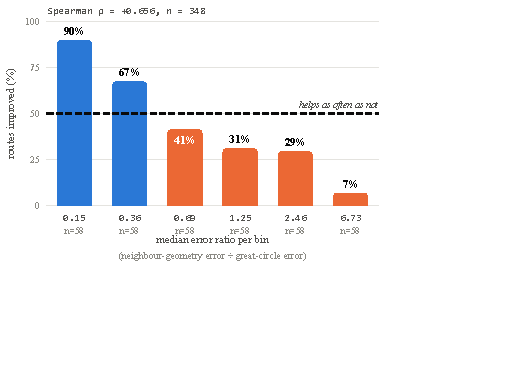
\includegraphics[width=\columnwidth]{fig2-error-ratio.pdf}
\caption{When corridor following helps, per route rather than per band. Above
the dashed line the method helps more often than not.}
\label{fig:ratio}
\end{figure}

The rule holds \emph{within} every length band, which makes it a statement
about the mechanism rather than about length, and it is the most directly
useful result here for anyone building such a router because it says in advance
when the method will fail. It is descriptive, not causal: the ratio and the
gain share the great-circle error as a denominator, so a route that is simply
hard to predict moves both. The binned pattern is the load-bearing part; the
correlation coefficient inherits that shared term and should not be read as an
effect size.

\subsection{Do cables avoid fishing grounds?}\label{sec:fishing}
External aggression---overwhelmingly fishing gear and anchors, in water
shallower than about 200\,m---accounts for roughly three quarters of recorded
cable faults~\cite{carter2009cables}. If cables are not following terrain, the
natural next hypothesis is that they are avoiding the hazard that actually
breaks them.

\begin{table}[t]
\caption{Fishing effort: mean percentile minus 50, by control displacement and
by how much of each route end is discarded. \textit{Positive means the cable
sits in heavier fishing than the water beside it.} $^{*}$~$p<0.05$ across
routes. The effect is confined to the untrimmed columns and vanishes at a
50\,km trim, which locates it at the landfalls.}
\label{tab:fishing}
\centering\footnotesize
\begin{tabular}{@{}lrrrr@{}}
\toprule
Displacement & No trim & 10\,km & 25\,km & 50\,km \\
\midrule
3\,km & \textbf{+0.90}$^{*}$ & \textbf{+1.34}$^{*}$ & \textbf{+1.30}$^{*}$ & +0.24 \\
5\,km & \textbf{+2.05}$^{*}$ & \textbf{+1.34}$^{*}$ & \textbf{+1.47}$^{*}$ & +0.15 \\
10\,km & +0.92 & +0.62 & +0.65 & $-$0.28 \\
20\,km & +0.86 & +0.11 & $-$0.43 & $-$0.50 \\
50\,km & +1.21 & +0.53 & $-$0.09 & $-$0.40 \\
\midrule
\textit{routes} & \textit{230} & \textit{203} & \textit{170} & \textit{141} \\
\bottomrule
\end{tabular}
\end{table}


\begin{figure}[t]
\centering
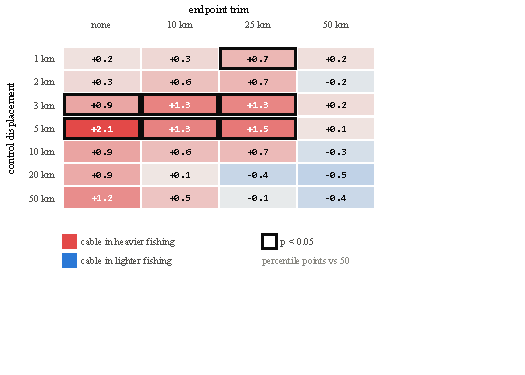
\includegraphics[width=\columnwidth]{fig3-fishing-sweep.pdf}
\caption{Fishing effect against endpoint trim and control displacement.
Outlined cells are significant across routes. The effect is confined to the
untrimmed and lightly trimmed columns and disappears at a 50\,km trim, which
locates it at the landfalls rather than along the route. The 1 and 2\,km rows
are shown for completeness but are not interpretable and are omitted from
Table~\ref{tab:fishing}: at $\sim$1.7\,km native resolution a control displaced
that far usually lands in the same cell and scores 50 by construction.}
\label{fig:fishing}
\end{figure}

\textbf{There is no fishing-avoidance signal} (Table~\ref{tab:fishing},
Fig.~\ref{fig:fishing}). What effect exists points the wrong way---cables in
slightly \emph{heavier} fishing---and it vanishes once 50\,km of each end is
removed. It is landfall geometry: coastal water is busy, and a perpendicular
control near shore moves offshore into quieter water. This is the same confound
that took the corridor effect from \nCorridorRaw\% to \nCorridorCtl\%. Depth
stratification agrees: at 5\,km displacement the effect is 54.6 on the shelf,
51.6 on the slope and 49.9 in deep water---confined to exactly the zone where a
coastal artefact would live, and absent where trawling avoidance would have to
show up if it were real.

\emph{One sub-design failed and is reported as untested rather than rejected.}
Cable protection zones restrict fishing near cables, so light fishing beside a
cable could be a \emph{consequence} of the cable. The displacement sweep was
designed to discriminate this---suppression predicts a step as the control
leaves the zone, route choice a smooth rise---but at $\sim$1.7\,km native
resolution a control displaced 1--2\,km usually lands in the same cell and
scores 50 by construction. A typical protection zone is narrower than one
native cell, and no resampling fixes that.

\section{Threats to Validity}\label{sec:threats}

\subsection{Measurement floor}
The flattest ruggedness quartile has local relief of 0.0--1.5\,m, the same
order as the downsampling error measured on those same shelf tiles
(0.46--1.28\,m RMS). Its near-null effect is partly an instrument limit, not
demonstrated absence of preference.

One source contradicts the main effect: DE~BSH-CONTIS shows cables on
\emph{steeper} ground ($\Delta$slope $+1.57$). It is also the only source whose
median terrain relief (1.0\,m) falls below the grid's own downsampling error
(1.28\,m RMS on shelf tiles). Measured across all sources, the
relief-to-noise ratio is 0.78 for BSH and 1.56--21.5 elsewhere, and every
source above the floor agrees with the main finding, the one sitting marginally
at the boundary agreeing most weakly. The contradiction tracks the measurement
floor, not the agency. We report this as a \emph{scope condition}---the method
needs relief above the bathymetry's noise---rather than as an unexplained
result.

\subsection{Scope and structure}\label{sec:scope}
\emph{Geographic coverage.} 75\% of corpus length is NW Europe and the
Mediterranean. The long-haul extension does not fix this; it \emph{sharpens}
it. The 2{,}000$+$\,km band is 13 of 15 routes from one agency and reduces in
practice to two corridors, transatlantic and Marseille--Levant, at $n=15$.
Broadening it needs as-laid geometry from non-European hydrographic offices,
which is a data-acquisition project rather than an analysis one.

\emph{Fold structure collapses above 1{,}000\,km.} Fewer than two sources reach
the eight-route minimum, so leave-one-source-out cannot run there. The
fixed-weight methods carry those results and need no fitting, but the spatially
blocked design that protects Section~\ref{sec:prediction} does not protect
Section~\ref{sec:longhaul}; the fitted method is reported as unavailable rather
than quietly fitted on the routes it is tested on.

\emph{Two resolutions are in play.} The coarser grid retains \nGateSlope\% of
the slope effect and \nGateRelief\% of relief (Table~\ref{tab:gate}), so
long-haul terrain results carry roughly half the sensitivity. This biases
\emph{against} terrain in the comparison where terrain loses, which is the
conservative direction, but it is not neutral and figures should not be quoted
across the two.

\emph{The corridor bound.} Bathymetry was loaded within $\pm 1^\circ$
($\sim$111\,km) of each route---generous for the median 171\,km route, tight
for the 49 routes over 1{,}000\,km, whose plausible alternatives may lie
outside it.

\emph{Regional $k$-sweep ambiguity.} In the regional band the $k$-sweep of
Section~\ref{sec:candidates} cannot cleanly separate ``removed the leak'' from
``removed the signal'', because a schematic entry for the subject and for its
genuine corridor-mates sit at similar distances. The long bands do not have
this problem.

\emph{Temporal direction.} The fishing surface is 2022 and most corpus cables
were laid earlier. Nothing in Section~\ref{sec:fishing} can establish that
planners avoided fishing grounds; at most it establishes that cables and
fishing effort are not spatially separated today.

\emph{Unmeasured criteria.} Bathymetry, existing infrastructure and fishing
intensity are measured here. Sediment type, anchoring zones, protected areas
and jurisdiction are not.

\section{Discussion}

\subsection{What the numbers say to a tool builder}
Cables do prefer flatter, less rugged seabed. The effect is real, controlled,
and consistent in sign across five of six independent national sources---and it
is small, and it does not scale with terrain difficulty in any way that
survives controlling for who published the data.

The most useful reading is the negative one: \textbf{bathymetry exerts a weak
influence on local cable position}, and the dominant factors are elsewhere. Of
the four candidate drivers weighed here---terrain, existing infrastructure,
fishing, and everything unmeasured---the second dominates, the first is small,
the third is absent, and a residual error of \nRegBoth\,km against a
\nDiscretisation\,km grid handicap says the fourth is still doing most of the
work: landing-point contracts, permitting, seasonal vessel availability and
commercial relationships.

This is a direct challenge to the premise of terrain-driven least-cost-path
cable routing. It does not make such tools useless---a route ignoring terrain
would be worse---but their output should be presented as one input to a
decision rather than as an optimum. Two consequences are specific enough to
act on:

\emph{Do not over-engineer the cost surface.} Fitting weights does not beat
guessing them. Effort spent learning a terrain cost function is better spent
elsewhere, which bears directly on the approach
of~\cite{google_patent_2021}.

\emph{Add the corridor term, and check the ratio first.} It is the strongest
single predictor found here, it needs no bathymetry, and
Section~\ref{sec:ratio} says in advance whether it will help on a given route.

\subsection{The corridor result has a policy counterpart}
Corridor reuse is not a neutral finding. Regulators and industry bodies have
examined \emph{spatial separation} of cables as a resilience
measure~\cite{csric2014separation}, on the reasoning that co-located systems
share fate under a single anchor drag or seabed event. Our measurement says
co-location is not merely permitted but is a strong empirical regularity in
where cables actually go, and that it grows stronger with distance. Whether
that reflects rational reuse of survey and permitting effort or an accumulating
concentration risk is outside what this dataset can answer, but the
quantification belongs in that debate.

\subsection{Reproducibility}\label{sec:repro}
Every number in this paper is produced by a script in the public
repository, writes its result to a cache, and is read from that cache by the
table and figure generators---so a figure or table disagreeing with the text
means one of them is stale rather than that a number was mistyped. The pipeline
requires no API key and no account; the only prerequisite is Node. Total
acquisition is about 615\,MB, most of it bathymetry, and after the cache is
built every test except the weight fit re-runs in under a minute combined.

The two load-bearing results are the cheapest to check. The corridor effect is
measured purely on route geometry and touches no bathymetry, so it needs the
corpus build alone---a couple of minutes, no tiles. The discretisation control,
which reversed the sign of the headline in Section~\ref{sec:prediction},
additionally needs the regional bathymetry.

\section{Conclusion}
We tested the premise underlying least-cost-path submarine cable routing
against \nCorpusRoutes{} as-laid routes and found it weak. Terrain preference
is real, small, does not strengthen with terrain difficulty once the publishing
agency is controlled for, and is captured as well by hand-set weights as by
fitted ones. A bathymetry-free alternative---proximity to existing
cables---outperforms it, survives four independent controls and a complete
replacement of its candidate set, strengthens with route length, and carries a
measured rule that predicts when it will fail. Fishing effort, the most
plausible remaining explanation, shows no signal at all.

Three controls made those findings possible, and each reversed or substantially
changed a headline: a placebo-displaced baseline, a discretisation penalty, and
a resolution gate. Their common lesson is that an evaluation of route-choice
models needs a stated zero point for its instrument, and neither the nominal
null, nor the analytic baseline, nor the finer grid the instrument was
calibrated on is automatically that zero point. Each has to be measured.

The obvious extension is geographic. The corpus is Europe-weighted because that
is where as-laid geometry is published; testing whether corridor reuse holds in
the Pacific, where cable systems are younger and corridors sparser, is a
data-acquisition problem and the single most valuable thing that could be done
next.

\section*{Acknowledgment}
This work uses open data published by EMODnet Human Activities, EMODnet
Bathymetry, and the NOAA National Centers for Environmental Information.

\bibliographystyle{IEEEtran}
\bibliography{refs}

\end{document}
